% Asset ID: A21DifferentiationTikZ-002
% Source: Chapter 9 worked example
% Related lesson section: Worked Example 2
% Purpose: Show stationary points of y = 1/2 x - cos(2x).
\documentclass[tikz,border=8pt]{standalone}
\usepackage{amsmath}
\usepackage{pgfplots}
\pgfplotsset{compat=1.18}
\begin{document}
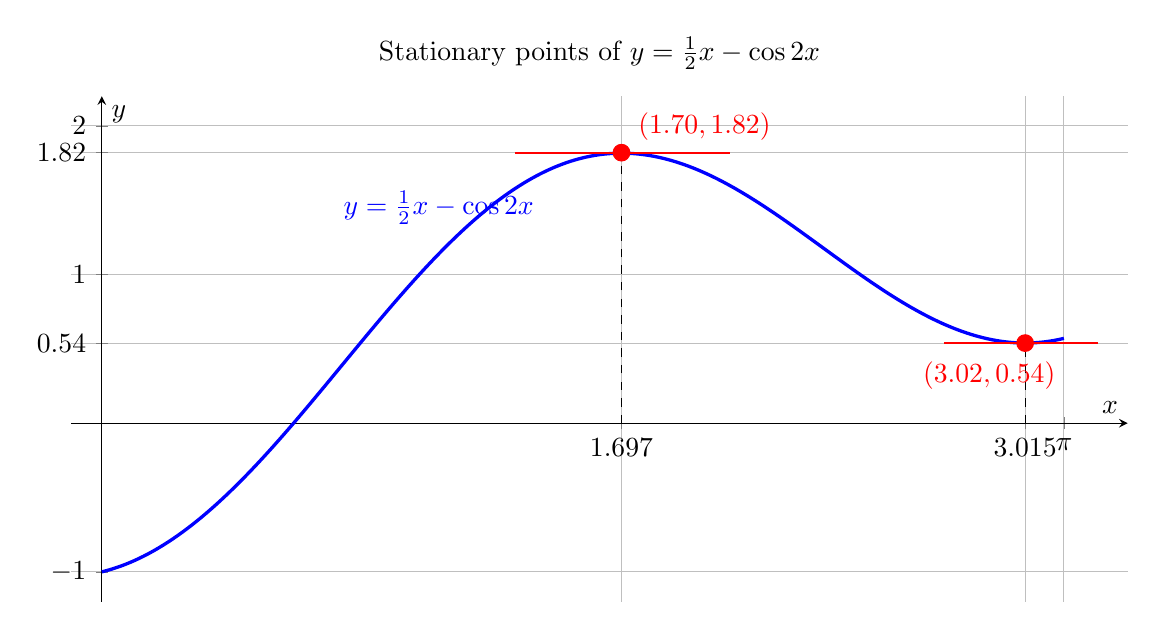
\begin{tikzpicture}
\begin{axis}[width=15cm,height=8cm,axis lines=middle,xmin=-0.1,xmax=3.35,ymin=-1.2,ymax=2.2,xtick={0,1.697,3.015,3.1416},xticklabels={$0$,$1.697$,$3.015$,$\pi$},ytick={-1,0,0.539,1,1.82,2},xlabel={$x$},ylabel={$y$},title={Stationary points of \(y=\frac12x-\cos 2x\)},samples=300,domain=0:3.1416,grid=both,minor tick num=1]
\addplot[very thick, blue] {0.5*x - cos(deg(2*x))};
\node[blue] at (axis cs:1.1,1.45) {$y=\frac12x-\cos 2x$};
\addplot[only marks, mark=*, mark size=3pt, red] coordinates {(1.697,1.82)(3.015,0.539)};
\addplot[red, thick, domain=1.35:2.05] {1.82};
\addplot[red, thick, domain=2.75:3.25] {0.539};
\draw[dashed] (axis cs:1.697,0) -- (axis cs:1.697,1.82);
\draw[dashed] (axis cs:3.015,0) -- (axis cs:3.015,0.539);
\node[red, anchor=south west] at (axis cs:1.72,1.84) {$(1.70,1.82)$};
\node[red, anchor=north west] at (axis cs:2.65,0.48) {$(3.02,0.54)$};
\end{axis}
\end{tikzpicture}
\end{document}
